In this section, we present our static program analysis algorithm for computing 
% an upper bound on the 
% execution-based reachability times 
the \emph{reachability-bound} for every program point $l$ in a program $c$ in a path sensitive manner.
% , as defined in last section.
%
% In order to have the upper bound of the reachability for every label of a program $c$, we design 
% a path sensitive reachability bound analysis algorithm {\THESYSTEM}.
The algorithm is summarized into the following steps,
% \begin{figure}
%   \centering    
% 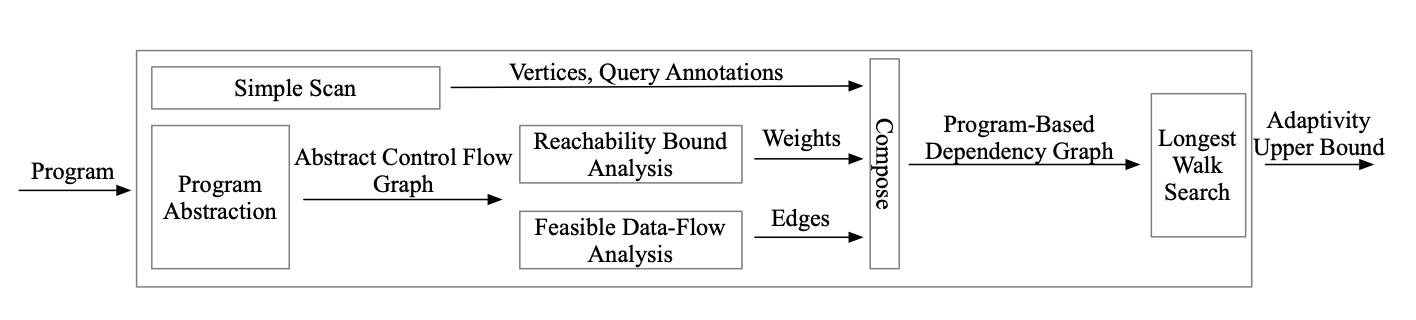
\includegraphics[width=1.0\columnwidth]{adapfun.png}
%   \vspace{-0.3cm}
%   \caption{The overview of {\THESYSTEM}}
%   \label{fig:adaptfun}
%   \vspace{-0.5cm}
% \end{figure}
%
\\
% \framebox{
    % \text{
    1. Compute Abstract Transition graph, $\absG(c)$ through program abstraction.
    % }
    \\
    % \text{
    2. Compute refined program by \cite{GulwaniJK09}, $\rprog$ for a program $c$ based on 
    its abstraction transition graph.
    \\
    3. Compute the Path-sensitive Reachability Bound $\psRB(c, l)$ in Section~\ref{sec:alg-rb} for every
    program location. 
    % }
% }
%
\begin{enumerate}
\item  The Section~\ref{sec:progabs} first 
computes the Abstract Transition graph, $\absG(c)$ for a program $c$ through program abstraction.
It computes the abstract transition 
for every labeled command in $c$ and each abstract transition is an edge in $\absG(c)$.
% This graph is used in the following sections
% %  from Section~\ref{sec:refine} to Section~\ref{sec:psrbcompute} 
% for computing the path-sensitive reachability-bound of a program location.
% see Section~\ref{sec:alg_vertexgen}
\item The second step in Section~\ref{sec:refine}
computes the refined program by the refine algorithm in \cite{GulwaniJK09}, $\rprog$ for a program $c$ based on 
its abstraction transition graph.
This algorithm transforms the multiple-paths loops
into multiple loops where
the interleaving of paths is explicit.
\item Section~\ref{sec:psrb} computes the path-sensitive reachability-bound for every program point.
It is based on computing the path reachability bound and the loop reachability bound
in Section~\ref{sec:looprb}.
The path reachability bound is an upper bound on the execution times of a transition path,
and
the loop reachability bound is an upper bound on the execution times of a outside loop 
w.r.t its nested loop. These two bounds also involve computing the ranking function  
\footnote{\textbf{ranking function} is the named used in \cite{SinnZV14}
and \textbf{local bound} is the name used in \cite{ZulegerGSV11}, \cite{sinn2017complexity}.
We refer to the two names as the same meaning in this paper.} 
for every transition path,
and estimates the upper bounds on every ranking function's maximum value. The details are in Section~\ref{sec:rank}.
\end{enumerate}
% Section~\ref{sec:rank} computes the ranking function  
% \footnote{\textbf{ranking function} is the named used in \cite{SinnZV14}
% and \textbf{local bound} is the name used in \cite{ZulegerGSV11}, \cite{sinn2017complexity}.
% We refer to the two names as the same meaning in this paper.} 
% for every transition path of the refined program,
% and estimates the upper bounds on every ranking function's maximum value.
